\chapter{System Requirements}
\label{chap:SysReq}

\section{Introduction}
\label{sec:SysReqIntro}
In this chapter we will present the system requirements, discovered both through conversation with the customer about their vision and through brainstorming sessions within the group. Since we were only given a limited vision of what the customer wanted, most requirements come from the brainstorming sessions. The system requirements are divided into functional and nonfunctional requirements and will be described in more detail through a series of use-cases at the end of this section.

\subsection{Definitions, Acronyms and Abbreviations}
\label{subsec:SysIntroReqDefs}

\subsubsection*{User}
A user is in this case the end-user of the web page. Since the web page is directed towards youth the typical end-user will be a teenager. 

\subsubsection*{Interactive Map}
The interactive map is Google Maps. In addition to navigate to different locations the map will in some cases show event information.

\subsubsection*{Tags}
A tag is in this case a word that helps describe a comment, picture, video or event. In this system all tags will be interests. 

\subsubsection*{Administrator}
An administrator is a person who is able to control and configure a part of a system or the entirety  of a system. In this system we envision two types of administrators, group administrators and system administrators. A group administrator is typically an end-user controlling a group page. A system administrator can control and make changes to the entire system.

\subsubsection*{Overview}
The system is a social platform urban youth to express themselves on. The users of the system will have the ability to upload pictures and videos to specific locations, host events and post comments. The system will be realized as a web page. After feedback from end users, we later decided to add a small Android application for uploading pictures to the system. This is discussed further elsewhere, most notably sections \ref{sec:S2Presentation} and \ref{sec:S4DesignImpl}. Requirements for both the website and the app are found in section \ref{sec:SysReqReqs}.

\subsection{Overall Description}
\label{subsec:SysReqIntroDescr}

At T\o yen in Oslo, a number of new outdoor places for youth are in the process of being built. As a part of that process, the researchers at AFI and the local politicians in the area wants input from the youth themselves. They want to see how the youth in the area express themselves both through picture and video uploads and through written comments. With this information they hope to get a better understanding of what can be done in order to improve the everyday life of the youth in the area. As well as being a source of information, the media uploads and comments will also create a social platform on its own where the youth can connect.
\subparagraph{} The system has four interfaces/parts:
\begin{itemize}
    \item Web Client (End users)
    \item Web Client (Administrators)
    \item Back end (Developers/Administrators)
    \item Android application (End users)
\end{itemize}

\subsection{User Characteristics}
\label{subsec:SysReqIntroUserChar}

As this system is aimed towards youth, most of the users will be between 12 and 20 years old. These are mostly users with prior experience of media sharing web pages and a user group that expects a certain level of intuitive design and functionality.

\subsection{Constraints}
\label{subsec:SysReqIntroConstr}

\subsubsection*{Time Constraints} 
This system will be developed over a short period of time. The resulting prototype will therefore be limited in functionality and design, but will contain the most important functionality. Some functionality will therefore have to be implemented at a later stage to have a fully functional system.
\subsubsection*{Assumptions and Dependencies} As the system we are developing is a web page with a database for storing user information and uploaded media, the system will always depend on an internet connection and an operational database. Because of moderation issues the system is also dependent on an administrator to remove potential inappropriate  media. The projects as a whole assume that the potential users will share the “correct” types of pictures and videos. “Correct” in this context can be pictures of interesting locations and videos of someone skating at a newly created skate ramp, while  “Incorrect” could be a lot of selfies.

\section{Non-functional and Functional Requirements}
\label{sec:SysReqReqs}

\subsection{Functional Requirements}
\label{subsec:SysReqReqsFunc}

\subsubsection{Sign in}
F1: A user should be able to sign up for a user profile. \\
F2: It should be possible to sign in and sign out.

\subsubsection{Search}
F3: It should be possible to search for events, pictures, comments and groups by using an interactive map and a search bar. \\
F4: It should be possible to add and delete search criteria in the search bar. \\
F5: A user should be able to zoom and move around in the interactive map. \\
F6: The interactive map should update according to the search criteria, showing the most relevant events in the specific area.

\subsubsection{Events}
F7: A user should be able to select events in the interactive map for more detailed event information. \\
F8: It should be possible to navigate to the event page of a specific event.\\
F9: A user should be able to see previously attended and upcoming events in a calendar.\\
F10: A registered user should be able to create and join events.\\
F11: The creator of an event should be able specify the location, activity and number of people who can join.

\subsubsection{Groups}
F12: It should be possible to create and join groups.\\
F13: The creator of a group, will also be the administrator of the group, with the possibility to accept/decline new group members, change the group description and remove undesirable pictures, videos and comments.

\subsubsection{Media Sharing}
F14: A registered user should be able to upload pictures and videos to specific locations on the interactive map and on group and event pages.\\
F15: The user should be able to attach interest- or group -tags to pictures the user wants to upload.\\
F16: The user should be able to click on an uploaded picture or video and get an enlarged version of the picture/video along with relevant information, such as title, description and location.

\subsubsection{Comments}
F17: A registered user should be able to comment on specific locations on the interactive map and on group and event pages. \\
F18: The user should be able to attach interest- or group -tags to a comment the user wants to post.

\subsubsection{Tags}
F19: The user should be able to suggest new interest-tags to be created.\\
F20: It should be possible to vote on suggested interest tags.\\
F21: When the number of votes for a specific interest tag has reached some set limit, the interest tag will be added if approved by the web page administrator.

\subsubsection{Rating}
F22: It should be possible to like or dislike a photo or an event.\\
F23: The user should be able to change a like to a dislike or the opposite.\\
F24: The user should be able to see whether or not he/she has voted on a photo earlier by highlighting the appropriate like or the dislike button.

\subsubsection{Android app sign in}
F25: It should be possible to sign in and sign out.

\subsubsection{Android app image uploading}
F26: The user should be able to take a new photo. \\
F27: The user should be able to browse images on the phone. \\
F28: The user should be able to upload a photo taken with the app, or uploaded from the phones gallery. \\
F29: All photos a user attempts to upload must be given a title, a description and interest tags. The photo also needs to be geotagged.


\subsection{Non-functional Requirements}
\label{subsec:SysReqReqsNonFunc}

\subsubsection{Usability}
\begin{itemize}
    \item The user should be able to learn the main functions of the website in a short amount of time.
    \item Intuitive user interface.
    \item The user should be able to connect to people with similar interests.
\end{itemize}

\subsubsection{Performance}
\begin{itemize}
    \item Minimal waiting time when user interacts with the web page.
\end{itemize}

\subsubsection{Security}
\begin{itemize}
    \item To upload pictures, create events, join events, post comments, suggest interest and vote for interests the user has to sign in with username and password.
    \item Usage of web page will be monitored by moderators.
\end{itemize}

\subsubsection{Availability}
\begin{itemize}
    \item The web page and back end of the system should always be available.
\end{itemize}

\subsubsection{Scalability}
\begin{itemize}
    \item The system should be able to support a large amount of users.
\end{itemize}

\subsection{Technical System Requirements}
\label{subsec:SysReqReqsTechnical}
The web page is compatible with all modern web browsers. These include Google Chrome, Firefox, Safari and Opera. For the front end of the page we use HTML version 5 and CSS version 3.

\paragraph{} As mentioned, mobile the application was made for Android. It was tested on phones with Android 4.4

\section{Use Cases}
\label{sec:SysReqUseCases}

A use case is a description or list of steps of what to do, in order to achieve a goal. It should define the interactions between an actor and the system itself. Here we present use cases with both textual descriptions and diagrams. The purpose of this is to get a better understanding of the system requirements and functions.

\subsection{Use Cases Related to the End Users}

\begin{minipage}{\linewidth}
\rowcolors{1}{blue!20}{blue!10}
\begin{tabular}{|l|p{85mm}|}
  \hline
  \multicolumn{2}{|c|}{\cellcolor{gray!25} \textbf{Sign in}} \\
  \hline
  Brief Description & The user should be able to sign in to the web page.\\
  Preconditions & The user must be a registered user with username and password. User also need an internet connection.\\
  Flow &
    \begin{enumerate}
      \item User clicks on “Sign in” button.
      \item User presented with a sign in page.
      \item User enters username and password.
    \end{enumerate} \\
  Basic flow & User enters user credentials and are logged in.\\
  Alternative Flows & The user enters invalid user credentials and has to try again.\\
  Special Requirements & \\
  Postconditions & The user is successfully logged in.\\
  Extension Points & \\
  \hline
\end{tabular}
\captionof{table}{Use case for sign in. \label{tab:SysReqUseCasesLogin}}
\end{minipage}

\begin{figure}[ht!]
\centering
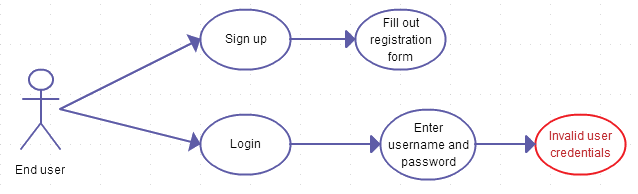
\includegraphics[width=105mm]{./SystemRequirements/img/loginUC.png}
\caption{Sign in use case \label{fig:SysReqUseCasesLogin}}
\end{figure}

\begin{minipage}{\linewidth}
\rowcolors{1}{blue!20}{blue!10}
\begin{tabular}{|l|p{85mm}|}
  \hline
  \multicolumn{2}{|c|}{\cellcolor{gray!25} \textbf{Search for event and media}} \\
  \hline
  Brief Description & The user should be able to search for events and media with location and interests as criteria.\\
  Preconditions & User needs internet connection.\\
  Flow &
    \begin{enumerate}
      \item User navigates to desired location in the interactive map.
      \item User enters interest tag in search bar.
      \item The search starts immediately
    \end{enumerate} \\
  Basic flow & User enter search criteria and finds relevant events and media. \\
  Alternative Flows & User only selects location.\\
  Special Requirements & \\
  Postconditions & The media feed is showing all relevant events and media. \\
  Extension Points & 
    \begin{itemize}
      \item 2a) User can add multiple interest tags to search. 
      \item 2b) User can remove interest tags from search. 
    \end{itemize} \\
  \hline
\end{tabular}
\captionof{table}{Use case for media search. \label{tab:SysReqUseCasesSearch}}
\end{minipage}

\begin{figure}[ht!]
\centering
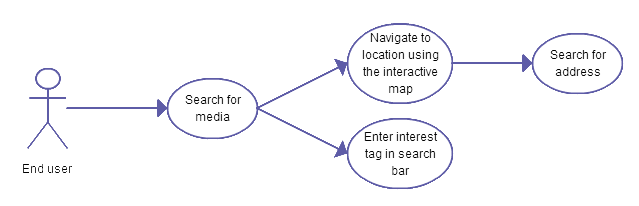
\includegraphics[width=105mm]{./SystemRequirements/img/searchUC.png}
\caption{Media search use case \label{fig:SysReqUseCasesSearch}}
\end{figure}

\begin{minipage}{\linewidth}
\rowcolors{1}{blue!20}{blue!10}
\begin{tabular}{|l|p{85mm}|}
  \hline
  \multicolumn{2}{|c|}{\cellcolor{gray!25} \textbf{Create event}} \\
  \hline
  Brief Description & The user should be able to create an event.\\
  Preconditions & The user must be logged in. User also needs an internet connection.\\
  Flow &
    \begin{enumerate}
      \item User clicks on “New event” button
      \item User writes a description of the event
      \item User sets location of the event
      \item User adds interest tag
      \item User sets maximal number of participants
    \end{enumerate} \\
  Basic flow & User navigates to the “new event” page, enters required specification of event, event is created.\\
  Alternative Flows & 
    \begin{itemize}
      \item 2a) User clicks on location in the interactive map and are presented with the option to create a new event there.
      \item 2b) User does not need to set the location if interest tag is added.
      \item 4a) User does not need add interest tag if location is set.
      \item 5a) User does not set number of participants.
    \end{itemize} \\
  Special Requirements & \\
  Postconditions & Users performing a search in the area of the event or with matching interest tag will see the created event in the media feed and in the interactive map.\\
  Extension Points & \\
  \hline
\end{tabular}
\captionof{table}{Use case for event creation. \label{tab:SysReqUseCasesEventCreate}}
\end{minipage}

\afterpage{
\clearpage
%\begin{landscape}
    \centering
    \begin{figure}
        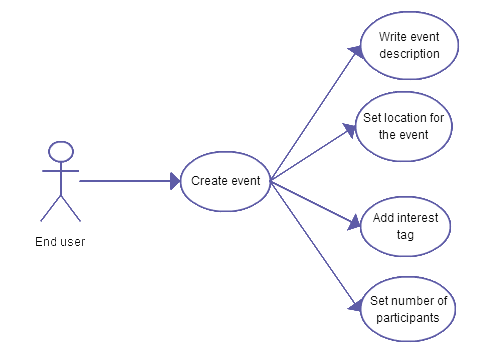
\includegraphics[width=100mm]{./SystemRequirements/img/eventUC.png}
        \caption{Event creation use case.}
        \label{fig:SysReqUseCasesEventCreate}
        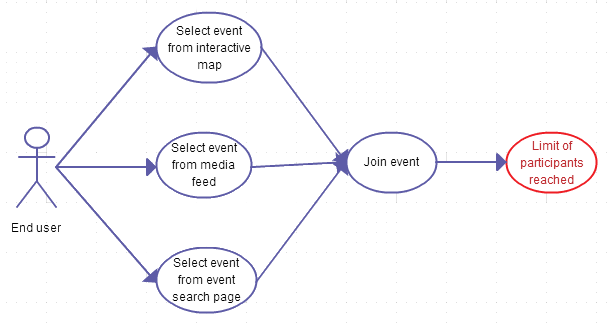
\includegraphics[width=100mm]{./SystemRequirements/img/joineventUC.png}
        \caption{Joining event use case.}
        \label{fig:SysReqUseCasesEventJoin}
    \end{figure}
%\end{landscape}
}


\begin{minipage}{\linewidth}
\rowcolors{1}{blue!20}{blue!10}
\begin{tabular}{|l|p{85mm}|}
  \hline
  \multicolumn{2}{|c|}{\cellcolor{gray!25} \textbf{Join event.}} \\
  \hline
  Brief Description & The user should be able to join a created event.\\
  Preconditions & The user must be a registered user with username and password.User needs an internet connection.\\
  Flow &
    \begin{enumerate}
      \item User selects event from the interactive map or the media feed.
      \item User presented with an event page with a more detailed description of the event.
      \item User clicks on join button.
    \end{enumerate} \\
  Basic flow & The user navigates to the event page of interest and joins the event by pressing a join button.\\
  Alternative Flows & 
    \begin{itemize}
      \item 3a) The number of participants has reached its set maximum and the join button does not show up.
    \end{itemize} \\
  Special Requirements & \\
  Postconditions & The number of participants are incremented by 1, and the event is added to the users calendar.\\
  Extension Points & \\
  \hline
\end{tabular}
\captionof{table}{Use case for joining events. \label{tab:SysReqUseCasesEventJoin}}
\end{minipage}

\begin{minipage}{\linewidth}
\rowcolors{1}{blue!20}{blue!10}
\begin{tabular}{|l|p{85mm}|}
  \hline
  \multicolumn{2}{|c|}{\cellcolor{gray!25} \textbf{Upload picture/video}} \\
  \hline
  Brief Description & The user should be able to upload pictures and videos to the web page for other users to see.\\
  Preconditions & The user need to be a registered user with username and password. User needs an internet connection.\\
  Flow &
    \begin{enumerate}
      \item User navigates to the upload media page.
      \item User clicks the “Browse” button.
      \item The user then needs to browse for the desired picture or video on the computer.
      \item The user adds an interest tag to the picture/video.
      \item The user clicks on the “Upload” button.
    \end{enumerate} \\
  Basic flow & The user navigates to the page for uploading different media, loads in the picture/video and adds interest tags to it before uploading it to the page.\\
  Alternative Flows & \\
  Special Requirements & \\
  Postconditions & The picture/video should now be available for other user to see. \\
  Extension Points & 
    \begin{itemize}
      \item 4a) The user can add multiple interest tags to the picture/video.
    \end{itemize} \\
  \hline
\end{tabular}
\captionof{table}{Use case for media upload. \label{tab:SysReqUseCasesMediaUpload}}
\end{minipage}

\begin{figure}
	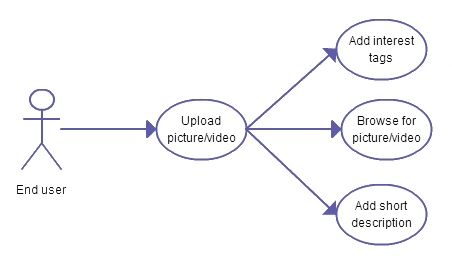
\includegraphics[width=95mm]{./SystemRequirements/img/uploadUC.png}
	\caption{Media upload use case. \label{fig:SysReqUseCasesMediaUpload}}
	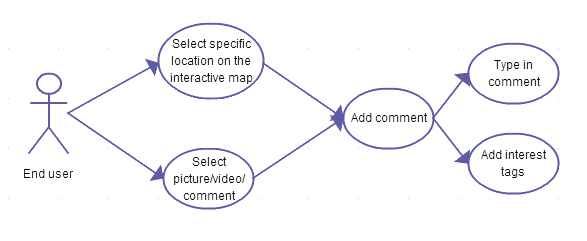
\includegraphics[width=105mm]{./SystemRequirements/img/commentUC.png}
	\caption{Commenting use case. \label{fig:SysReqUseCasesComment}}
\end{figure}


\begin{minipage}{\linewidth}
\rowcolors{1}{blue!20}{blue!10}
\begin{tabular}{|l|p{85mm}|}
  \hline
  \multicolumn{2}{|c|}{\cellcolor{gray!25} \textbf{Post a comment}} \\
  \hline
  Brief Description & The user should be able to post comments on locations in the map and comment on media and other comments.\\
  Preconditions & The user must be a registered user with username and password. User also need an internet connection.\\
  Flow &
    \begin{enumerate}
      \item User clicks on a specific location in the interactive map.
      \item User presented with the option to comment on the location.
      \item User clicks on “Add comment”
      \item User presented with other comments posted in a small radius around the location. 5) Gets the option to create a separate comment or comment on one of the already existing comments.
      \item User selects to create a separate comment.
      \item User presented with a text field for the comment.
      \item User adds an interest tag to the comment.
      \item User enters comment and clicks on “Post comment”.
    \end{enumerate} \\
  Basic flow & The user selects a location in the interactive map and chooses to add a new comment there. The user then writes the comment and posts it.\\
  \hline
\end{tabular}
\end{minipage}

\begin{minipage}{\linewidth}
\begin{tabular}{|l|p{85mm}|}
  \hline
  Alternative Flows & 
    \begin{itemize}
      \item 1a) User clicks on an image,video or comment.
      \item 4a) User not presented with other comments if there are no comments in the area.
      \item 6a) User selects to comment on an already existing comment.
      \item 8a) User does not need to add an interest tag.
    \end{itemize} \\
  Special Requirements & \\
  Postconditions & The comment is made available for the other users to see.\\
  Extension Points & The user can add multiple interest tags to a new separate comment.\\
  \hline
\end{tabular}
\captionof{table}{Use case for commenting. \label{tab:SysRecUseCasesComment}}
\end{minipage}

\begin{figure}[ht!]
\centering
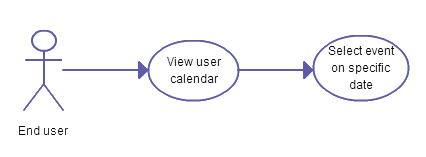
\includegraphics[width=105mm]{./SystemRequirements/img/preveventUC.png}
\caption{Previous event use case \label{fig:SysReqUseCasesEventPrev}}
\end{figure}

\begin{minipage}{\linewidth}
\rowcolors{1}{blue!20}{blue!10}
\begin{tabular}{|l|p{85mm}|}
  \hline
  \multicolumn{2}{|c|}{\cellcolor{gray!25} \textbf{Find previously attended  event page}} \\
  \hline
  Brief Description & The user should be able to find the event pages to the events the user has attended. \\
  Preconditions & \\
  Flow &
    \begin{enumerate}
      \item User clicks on the calendar.
      \item User presented with a calendar showing the current month.
      \item User navigates to the previous month in the calendar.
      \item User presented with all attended events in the calendar.
      \item User selects one of the events.
      \item User presented with the event page for that event.
    \end{enumerate} \\
  Basic flow & The user clicks on the calendar, maneuvers to the desired date and selects the event showing up at that date. The user are then brought to the selected event page. \\
  Alternative Flows & \\
  Special Requirements & \\
  Postconditions & The previously attended event page are showing.\\
  Extension Points & \\
  \hline
\end{tabular}
\captionof{table}{Use case for finding previously attended events. \label{tab:SysReqUseCasesEventPrev}}
\end{minipage}

\begin{minipage}{\linewidth}
\rowcolors{1}{blue!20}{blue!10}
\begin{tabular}{|l|p{85mm}|}
  \hline
  \multicolumn{2}{|c|}{\cellcolor{gray!25} \textbf{Suggest new interest tag}} \\
  \hline
  Brief Description & The user should be able to suggest a new interest.\\
  Preconditions & The user must be a registered user with username and password. User needs an internet connection. The new interest tag should not exist.\\
  Flow &
    \begin{enumerate}
      \item User enters interest into search bar.
      \item User informed that the entered interest does not exist.
      \item User presented with option of suggesting the interest as a new interest tag.
      \item User choosing the option to suggest as new tag.
    \end{enumerate} \\
  Basic flow & User tries to search with non existing interest tag, gets informed, suggests the interest tag as a new tag.\\
  Alternative Flows & 
    \begin{itemize}
      \item 1a) User tries to attach an interest tag to a picture, video or comment.
    \end{itemize} \\
  Special Requirements & \\
  Postconditions & The suggested interest tag is added to the list of suggested interest tags, on the suggested interest tags page.\\
  Extension Points & \\
  \hline
\end{tabular}
\captionof{table}{Use case for suggesting interest tags. \label{tab:SysReqUseCasesSuggestTag}}
\end{minipage}

\begin{figure}[ht!]
\centering
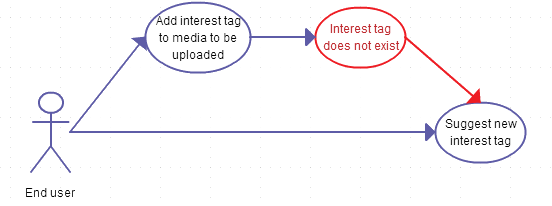
\includegraphics[width=105mm]{./SystemRequirements/img/suggesttagUC.png}
\caption{Suggest interest tag use case \label{fig:SysReqUseCasesSuggestTag}}
\end{figure}

\begin{minipage}{\linewidth}
\rowcolors{1}{blue!20}{blue!10}
\begin{tabular}{|l|p{85mm}|}
  \hline
  \multicolumn{2}{|c|}{\cellcolor{gray!25} \textbf{Vote on suggested interest tag}} \\
  \hline
  Brief Description & The user should be able to vote on a suggested interest tag.\\
  Preconditions & The user must be a registered user with username and password. User needs an internet connection.\\
  Flow &
    \begin{enumerate}
      \item User clicks on “Suggested interests” button.
      \item User presented with a list of interest tags the suggested interests page.
      \item User clicks on “vote” beside the desired tag.
    \end{enumerate} \\
  Basic flow & User navigates to the suggested interests page, and votes on desired tags.\\
  Alternative Flows & \\
  Special Requirements & \\
  Postconditions & The tag the user chose to vote on, has one more vote.\\
  Extension Points & \\
  \hline
\end{tabular}
\captionof{table}{Use case for interest tag voting. \label{tab:SysReqUseCasesVoteTag}}
\end{minipage}

\begin{figure}[ht!]
\centering
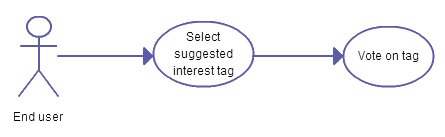
\includegraphics[width=105mm]{./SystemRequirements/img/votetagUC.png}
\caption{Vote on interest tag use case \label{fig:SysReqUseCasesVoteTag}}
\end{figure}